\documentclass[a4paper,12pt]{article}

% Pakete für zusätzliche Funktionen
\usepackage[utf8]{inputenc}   % UTF-8 Zeichencodierung
\usepackage[T1]{fontenc}     % Korrekte Silbentrennung und Umlaute
\usepackage[ngerman]{babel}  % Deutsche Spracheinstellungen
\usepackage{amsmath, amssymb} % Mathematische Symbole
\usepackage{graphicx}        % Einfügen von Bildern
\usepackage{hyperref}        % Hyperlinks
\usepackage{geometry}        % Seitenränder
\usepackage{listings}        % Code-Listings
\usepackage{csquotes}        % Zitate
\usepackage{csvsimple}  % Für das Einfügen von CSV-Dateien
\usepackage{titlesec}
\usepackage{float}  % Add this to your preamble
\newcommand{\sectionbreak}{\clearpage}
\geometry{a4paper, margin=2.5cm}
% Einstellungen für Hyperlinks
\hypersetup{
    colorlinks=true,
    linkcolor=blue,
    citecolor=blue,
    filecolor=magenta,
    urlcolor=cyan,
    pdftitle={Implementierung digitaler Geschäftsprozesse},
    pdfpagemode=FullScreen,
}

% Titel und Autoreninformationen
\title{\textbf{Implementierung digitaler Geschäftsprozesse}}
\author{Kürsat Darcan | MFWS422A}
\date{Abgabedatum: \today}

\begin{document}

% Deckblatt
\maketitle
\thispagestyle{empty}
\vspace{2cm}
\begin{center}
    \includegraphics[width=0.3\textwidth]{FHDW_Logo_RGB-01.svg.png} % Ersetzen Sie "example-image" durch Ihr Logo/Bild
    \\
    \vspace{1cm}
    \textbf{Studiengang: Wirtschaftsinformatik}\\
    \textbf{Fachhochschule der Wirtschaft (FHDW)}
\end{center}
\newpage

% Inhaltsverzeichnis
\renewcommand{\thepage}{\roman{page}} % Seitenzahlen in römischen Ziffern für Verzeichnisse
\tableofcontents
\newpage

% Bei Bedarf Abbildungsverzeichnis
\listoffigures
\addcontentsline{toc}{section}{Abbildungsverzeichnis}
\newpage

% Bei Bedarf Tabellenverzeichnis
\listoftables
\addcontentsline{toc}{section}{Tabellenverzeichnis}
\newpage
%-- Beispiel für eine Tabelle --%
%\begin{table}[htbp]
%    \centering
%    \resizebox{\textwidth}{!}{ 
%    \csvautotabular[separator=semicolon]{tabellen/scm1/test.csv}  % Pfad zur CSV-Datei
%    }
%    \caption{Beispieltabelle aus test.csv}
%    \label{tab:testcsv}
%\end{table}
%-- Ende Beispiel --%

% Abkürzungsverzeichnis
\section*{Abkürzungsverzeichnis}
\addcontentsline{toc}{section}{Abkürzungsverzeichnis}
\begin{description}
    \item[CRM] Customer Relationship Management
    \item[SCM] Supply Chain Management
\end{description}
\newpage

% Hauptteil mit arabischen Seitenzahlen
\renewcommand{\thepage}{\arabic{page}} % Seitenzahlen in arabischen Ziffern für den Hauptteil
\setcounter{page}{1}


% Einleitung
\section{Einleitung}
\subsection{Zielsetzung der Ausarbeitung}
Diese Ausarbeitung ist Teil des Moduls \textbf{Implementierung digitaler Geschäftsprozesse}.
Die Ausarbeitung bildet den Ablauf und die Reflexion des Planspiels \textit{kdibisglobal} ab,
das im Rahmen des Moduls durchgeführt wurde.
Hierbei wird auf die einzelnen Spielrunden eingegangen
und die jeweiligen Ergebnisse und Erkenntnisse analysiert und reflektiert.
Zusätzlich werden weitere Methoden
erläutert, die im Rahmen des Moduls behandelt wurden, aber nicht im Planspiel angewendet werden konnten.

\subsection{Überblick über das Planspiel kdibisglobal}
\textbf{kdibisglobal} wurde speziell für das Buch Integrierte Business-Informationssysteme von Herrn Klaus-Dieter Gronwald entwickelt,
um ein praktisches Verständnis für digitale Geschäftsprozesse zu erlangen.
Das Planspiel simuliert das Geschäftsprozessmanagement für einen Bierhersteller.

In diesem Planspiel übernehmen die Teilnehmer einzelne Bereiche innerhalb des Unternehmens und sind für die jeweiligen Bestellungen zuständig.
Dabei müssen verschiedene Faktoren berücksichtigt werden, wie Lieferverzögerungen, Verfügbarkeit von Produkten, saisonale Nachfrage und so weiter.
Zusätzlich werden wichtige Bereiche wie Supply Chain Management (SCM) und Customer Relationship Management (CRM) abgebildet.

Im Rahmen des SCM geht es darum, Bestände sinnvoll zu planen, Nachbestellungen rechtzeitig auszulösen und Lieferengpässe zu vermeiden.
Beim CRM steht die Beziehung zum Kunden im Vordergrund, also etwa das Management von Aufträgen,
die Sicherstellung einer hohen Kundenzufriedenheit sowie die Reaktion auf Änderungen in der Nachfrage.

Ziel ist es, durch den richtigen Einsatz digitaler Systeme die Unternehmensprozesse effizient zu gestalten.\cite{Kdibisglobal2025}

% Ablauf und Reflexion des Planspiels
\section{Ablauf und Reflexion des Planspiels}
Die Erkenntnisse sowie die Ergebnisse des Planspiels werden in drei Spielrunden unterteilt und analysiert.
Zusätzlich werden die theoretischen Inhalte aus dem Modul Implementierung digitaler Geschäftsprozesse erläutert und
in den Kontext des Planspiels gesetzt.

Für die Spielrunden SCM1 und SCM2 wird das Supply Chain Management nur im Bereich des Einzelhandels betrachtet,
da der Autor der Ausarbeitung hierfür zuständig war.

Für die Spielrunde CRM2 wird das Customer Relationship Management betrachtet. Da jedes Teammitglied einen Einzelhandel repräsentiert hat, also 5 Teammitglieder auf 4 Einzelhandel verteilt wurden,
mussten der Autor und ein weiteres Teammitglied gemeinsam für Einzelhandel 1 agieren. Jeder Einzelhandel hatte bis zu 12 Produkte. Da in Einzelhandel 1 zwei Teammitglieder zuständig waren, mussten die Produkte durch 2 aufgeteilt werden.
Dem entsprechend kann nicht das gesamte Einzelhandelsproduktsortiment betrachtet werden, sondern nur die Produkte, für die der Autor zuständig war.

\subsection{Spielrunde 1 – SCM1: Bullwhip Game und ERP-Strategie}
SCM 1 ist die erste Spielrunde, in dem ein Jahr simuliert wird unnd eine Bestellzyklus von 1 Woche besteht, was 52 Spielrunden entspricht.
Zudem gibt es in diesem Spieljahr keinen Forecast, kein Inventory Management und keine Kommunikation zwischen den Teammitglieder.
Ziel ist es dabei die Auswirkungen eines nicht kommunikativen Supply Chain Management zu erfahren und eine Demonstration des Bullwhip-Effekts zu erfahren.
--Quelle--

Nachdem die  erste spielrunde erläuert wurde, wird auf die einzelnen Spielrunden eingegangen.
%\begin{table}[H]
%    \centering
%    \resizebox{\textwidth}{!}{ 
%    \csvautotabular[separator=semicolon]{tabellen/scm1/scm1komplettablauf.csv}  % Pfad zur CSV-Datei
%    }
%    \caption{SCM 1 Spielablauf}
%    \label{tab:SCM 1 Spielablauf}
%\end{table}

Wie aus der Tabelle zu entnehmen ist, verliefen die ersten 10 Spielrunden sehr erfolgreich, und die Bestellungen wurden stets rechtzeitig ausgelöst.
Zusätzlich konnte die Lagerhaltung konstant bei durchschnittlich 1000 hl gehalten werden.

Ab Woche 11 kam es jedoch zu plötzlichen Lieferverzögerungen, die durch die Simulation verursacht wurden.
Trotz der Regeln des Planspiels ließ sich die Ursache der Verzögerungen nicht feststellen, da zu diesem Zeitpunkt keine Kommunikation zwischen den Teammitgliedern stattfinden konnte.
Infolge der Lieferprobleme konnten die Bestellungen an die Einzelhändler nicht vollständig ausgeliefert werden, wodurch bis Woche 14 Fehlmengen von bis zu 9000 hl auftraten.

Zudem führte Unerfahrenheit zu mehreren Überbestellungen in den Wochen 13 und 14.
Hätte sich die Überbestellung nur auf Woche 13 beschränkt, wären die Auswirkungen auf die Lagerhaltung gering gewesen,
da dadurch die Fehlmengen der Wochen 12 bis 14 ausgeglichen worden wären und ein Lagerbestand von über 4000 hl erzielt worden wäre.
Die zusätzlichen Bestellungen in Woche 14 bewirkten jedoch, dass der Lagerbestand in Woche 17 auf über 15000 hl anwuchs.
Dies verursachte hohe Lagerkosten, die erst bis Woche 23 durch den Bestelleingang teilweise ausgeglichen werden konnten.
In diesem Zeitraum kam es zu Bestellungen mit weniger als 1000 hl, wodurch der Bullwhip-Effekt deutlich erkennbar wurde.

Fehlkalkulationen und der Bullwhip-Effekt führten zu emotionalen Reaktionen: Lagerbestände sowie Bestell- und Auslieferungsprozesse wurden zunehmend unachtsam gehandhabt.
In den Wochen 24 bis 26 entstanden dadurch weitere Fehlmengen, die aufgrund unüberlegter Bestellungen nicht mehr ausgeglichen werden konnten.

Zwischen Woche 26 und Woche 36 stabilisierte sich die Situation, und Lagerbestände sowie Bestellungen konnten wieder besser aufeinander abgestimmt werden.

In den Wochen 37 bis 52 bestand das Ziel darin, Fehlmengen zu vermeiden und stets einen ausreichenden Lagerbestand vorzuhalten,
um vollständige Auslieferungen zu gewährleisten.
Allerdings führte dieses Ziel zu erneut hohen Lagerkosten, verursacht durch Überbestellungen im Verlauf der Wochen ab Woche 37.
Auch hier kam es wieder zu emotional gesteuerten Bestellungen, die ohne sorgfältige Berücksichtigung des tatsächlichen Bestelleingangs ausgelöst wurden, lediglich um Fehlmengen zu verhindern.

%\begin{figure}[H]
%    \centering
%    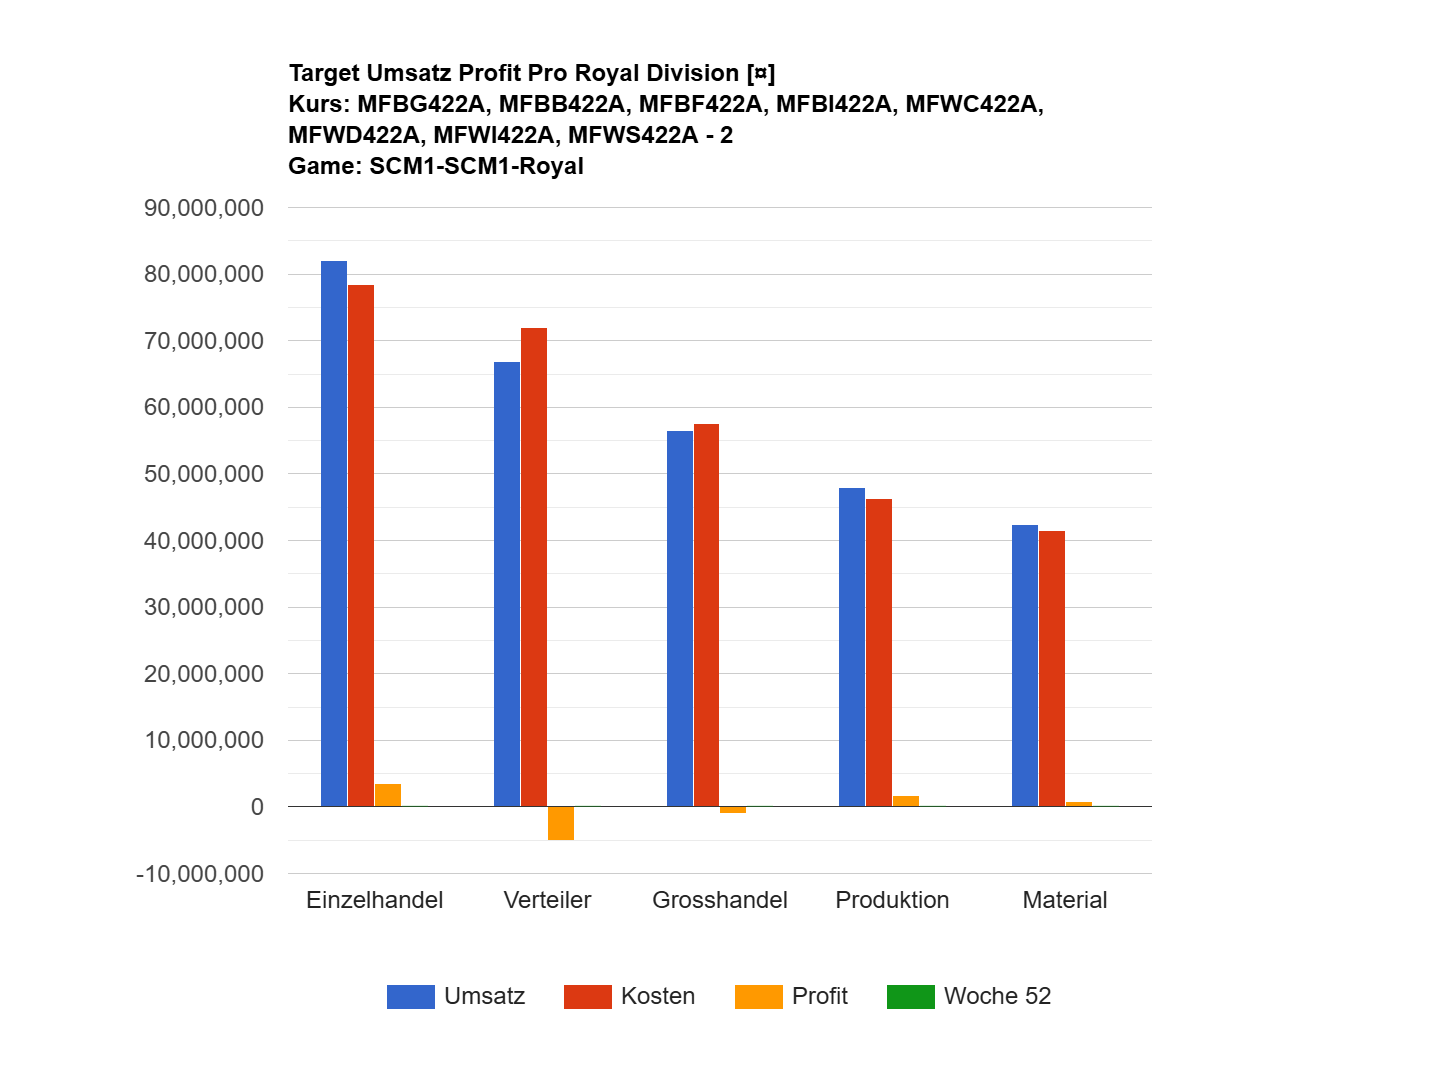
\includegraphics[width=0.7\textwidth]{abbildungen/scm1/scm1Umsatz.png}
%    \caption{SCM1 Umsatz}
%    \label{fig:SCM1 Umsatz}
%\end{figure}

Dennoch ist deutlich anhand des Abbilds zu erkennen, dass die Umsätze für den Einzelhandel mehr als 3,5 Millionen Euro betrugen
und der Bullwhip-Effekt keinen großen Einfluss auf den Umsatz hatte, wie in den anderen Unternehmensbereichen.

\subsubsection{Ursachen des Bullwhip-Effekts im Planspiel}
Nun wurde mehr mals erwähnt, dass der Bullwhip-Effekt aufgetreten ist.
Was genau bedeuetet den Bullwhip-Effekt, wie kommt dieser zustande und wie kann dieser vermieden werden?
%\begin{figure}[H]
%    \centering
%    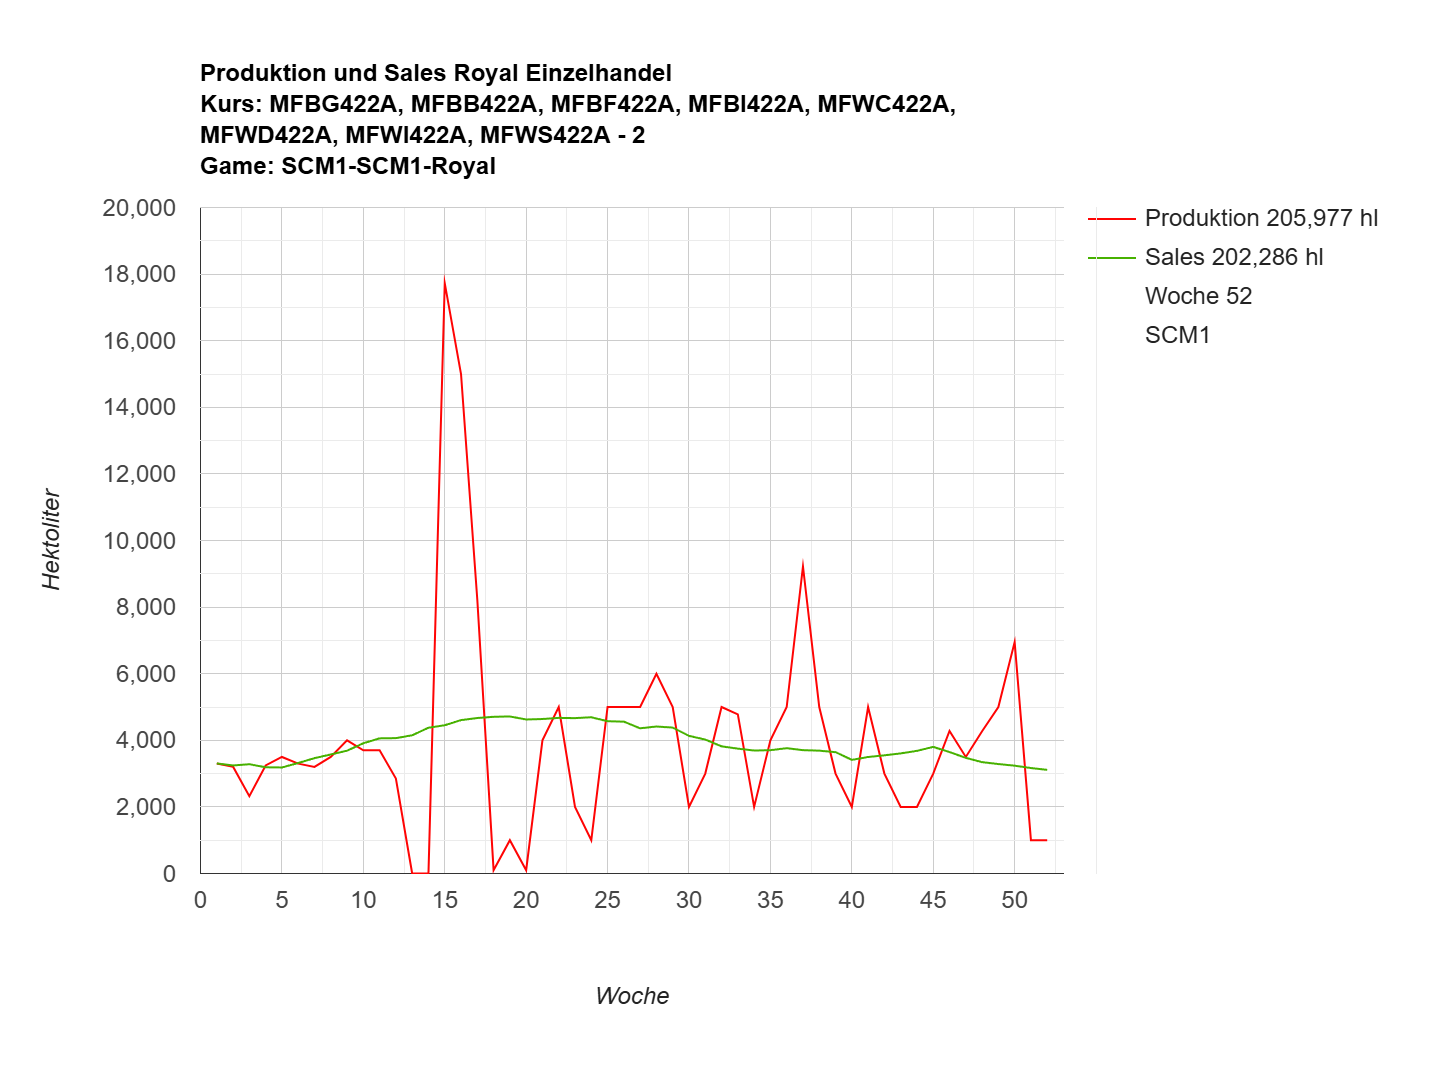
\includegraphics[width=0.7\textwidth]{abbildungen/scm1/scm1bullwhipeffektindex.png}
%    \caption{SCM1 Bullwhip-Effekt-Index}
%    \label{fig:SCM1 Bullwhip-Effekt-Index}
%\end{figure}
Auch soll die Abbildung \ref{fig:SCM1 Bullwhip-Effekt-Index} verdeutlichen, wie stark der Bullwhip-Effekt ausgeprägt sein kann.
Wie setzt sich der Bullwhip-Effekt zusammen? Zum einen, wie in Kapitel Spielrunde 1 erläutert, liegt es an mangelnder Kommunikation zwischen den Teammitgliedern,
 zum anderen an fehlender Transparenz zwischen den Bereichen.
Zudem spielen weitere Faktoren eine Rolle, wie zum Beispiel Demand Signal Processing, das bei saisonaler Nachfrage zu Überreaktionen oder Fehleinschätzungen führen kann.
Auch Order Batching oder eine lange Lead Time können den Bullwhip-Effekt deutlich verstärken.
Das bedeutet: Wenn Abteilungen Bestellungen auf- oder abrunden, kommt es zu stärkeren Verzerrungen der Bestellmengen.
Bei der Lead Time spielt die Zeitdifferenz zwischen Bestellung und Erhalt der Ware eine entscheidende Rolle.
Wenn Teammitglieder auf die Supply Chain reagieren, die Waren jedoch verzögert eintreffen, kann ein starker Effekt entstehen, wie es in den Wochen 11–18 aufgetreten ist und in Abbildung \ref{fig:SCM1 Bullwhip-Effekt-Index} erkennbar ist.

\subsubsection{IT-Situation der Einzelhandelsketten 1–4}
\subsubsection{Wahl einer M\&A IT-Integrationsstrategie}
\subsubsection{Organisational Readiness und CMMI-Reifegrade}

\newpage
\subsection{Spielrunde 2 – SCM2: Forecasting und Inventory Management}
\subsubsection{Bestell- und Lieferverhalten im Einzelhandel}
\subsubsection{Teamstrategie und interne Abstimmung}
\subsubsection{Auswahl und Anwendung von Forecastingmethoden}
\subsubsection{Optimierung der Bestellkosten im Einzelhandel}
\subsubsection{Umgang mit Lieferverzögerungen über Blockchain \& Smart Contracts}
\subsubsection{Anwendung des Kanban-Prinzips zur Optimierung der Lieferkette}

\newpage
\subsection{Spielrunde 3 – CRM3: Kundenmanagement mit Big Data}
\subsubsection{Analyse der Einzelhandels-Ergebnisse im 3. Fiskaljahr}
\subsubsection{ Performance-Analyse mit Word Tree \& beworbenen Produkten}
\subsubsection{Einsatz von Sentiment Analysis im CRM und Marketing}

\newpage
% Fazit
\section{Fazit}
\subsection{Wichtige Erkenntnisse für den Einzelhandel aus den Spielrunden}
\subsection{Bewertung des eigenen Verhaltens und der Teamkoordination}

% Literaturverzeichnis
\newpage
\addcontentsline{toc}{section}{Literaturverzeichnis}
\section*{Literaturverzeichnis}
\begin{thebibliography}{99}
    \bibitem{Gronwald2020} Gronwald, (2020). \textit{Integrierte Business-Informationssysteme – Ganzheitliche, geschäftsprozessorientierte Sicht auf die vernetzte Unternehmensprozesskette ERP, SCM, CRM, BI, Big Data Analytics}. Springer Vieweg, 2020. Verfügbar unter: \url{https://link.springer.com/book/10.1007/978-3-662-59815-3} (zuletzt aufgerufen am 27.04.2025)
    \bibitem{Kdibisglobal2025} Gronwald, K.D. \textit{kdibisglobal – Planspiel zur Umsetzung integrierter Business-Informationssysteme}. Verfügbar unter: \url{https://www.kdibisglobal.org/php/kdiglobstart.php} (zuletzt aufgerufen am 27.04.2025)
\end{thebibliography}


\newpage
% Anhang
%\appendix
%\section{Anhang}
%Hier können zusätzliche Informationen, wie Code-Beispiele oder ausführliche Tabellen, eingefügt werden.

% Ehrenwörtliche Erklärung
\newpage
\addcontentsline{toc}{section}{Ehrenwörtliche Erklärung}
\section*{\texttt{Ehrenwörtliche Erklärung}}
Hiermit erkläre ich, dass ich die vorliegende schriftliche Ausarbeitung im Modul \textbf{Implementierung digitaler Geschäftsprozesse} selbstständig
angefertigt habe. Es wurden nur die in der Arbeit ausdrücklich benannten Quellen und
Hilfsmittel benutzt. Wörtlich oder sinngemäß übernommenes Gedankengut habe ich als
solches kenntlich gemacht. Diese Arbeit hat in gleicher oder ähnlicher Form noch keiner
Prüfungsbehörde vorgelegen.

\vspace{3cm}
\noindent\begin{tabular}{p{0.5\textwidth}p{0.5\textwidth}}
    \hrulefill & \hrulefill \\
    Ort, Datum & Unterschrift \\
\end{tabular}

\end{document}
